% Load the kaohandt class (with the default options)
\documentclass[
	%fontsize=10pt, % Base font size
	%twoside=false, % If true, use different layouts for even and odd pages (in particular, if twoside=true, the margin column will be always on the outside)
	%secnumdepth=2, % How deep to number headings. Defaults to 2 (subsections)
	%abstract=true, % Uncomment to print the title of the abstract
]{kaohandt}

% Choose the language
\usepackage[english]{babel} % Load characters and hyphenation
\usepackage[english=british]{csquotes}	% English quotes

% Load packages for testing
\usepackage{blindtext}
% \usepackage{showframe} % Uncomment to show boxes around the text area, margin, header and footer
%\usepackage{showlabels} % Uncomment to output the content of \label commands to the document where they are used

\graphicspath{{images/}{./}} % Paths where images are looked for

% Load mathematical packages for theorems and related environments.
\usepackage{kaotheorems}

% Load the bibliography package
\usepackage{kaobiblio}
\addbibresource{main.bib} % Bibliography file

% Load the package for hyperreferences
\usepackage{kaorefs}
% \usepackage{authblk}

% \usepackage{nomencl}
% \makenomenclature

%----------------------------------------------------------------------------------------

\begin{document}

%----------------------------------------------------------------------------------------
%	REPORT INFORMATION
%----------------------------------------------------------------------------------------

\title[Numerical optimization of aviation decarbonization scenarios]{\textbf{Supplementary Information}
\bigskip

\textit{Numerical optimization of aviation decarbonization scenarios: balancing traffic and emissions with maturing energy carriers and aircraft technology}}


% \author[1,2]{Ian Costa-Alves}
% \author[1]{Nicolas Gourdain}
% \author[2]{François Gallard}
% \author[2]{Anne Gazaix}
% \author[1,3]{Yri Amandine Kambiri}
% \author[3]{Thierry Druot}

\author[ICA, NG, FG, AG, YK, TD]{Ian Costa-Alves \thanks{Aerodynamics, Energetics, and Propulsion Department, ISAE-SUPAERO}\ \thanks{Center of Competence on Multidisciplinary Design Optimization, IRT Saint Exupéry} \\ Nicolas Gourdain \footnotemark[1] \\ François Gallard \footnotemark[2] \\ Anne Gazaix\footnotemark[2] \\ Yri Amandine Kambiri \footnotemark[1]\ \thanks{Conceptual Airplane Design and Operations, ENAC, Toulouse, France} \\ Thierry Druot \footnotemark[3]}

\bigskip

\date{\today}

%----------------------------------------------------------------------------------------
%	TITLE AND ABSTRACT
%----------------------------------------------------------------------------------------

\maketitle

\margintoc

\begin{abstract}
\noindent
Supplementary information regarding the equations and their calibration methodology behind the mathematical models (optimization controls, demand, aircraft, fleet, energy), and the full results of all the simulated scenarios.
\end{abstract}


% {\noindent\textbf{Keywords:} System Dynamics, Multi-Disciplinary Optimization, Policy Optimization, Model Calibration, Numerical Methods}


%----------------------------------------------------------------------------------------
%	MAIN BODY
%----------------------------------------------------------------------------------------
\newpage

\section*{Variables}

\begin{center}
\footnotesize
\begin{tabular}{l l}
\toprule
Symbol & Description \\
\midrule
$o$ & Delay output variable \\
$i$ & Delay input variable \\
$\tau$ & Delay-time (time constant) \\
$D$ & Aggregate demand \\
$Pop$ & Population \\
$I$ & Per-capita income \\
$p$ & Ticket price \\
$\epsilon_{\upsilon}$ & Elasticity of demand to variable $\upsilon$ \\
$\sigma$ & Calibration constant \\
$RPKpc_{trend}$ & Trend per-capita Revenue Passenger Kilometers \\
$L$ & Left asymptote (propensity to travel at zero income) \\
$R$ & Right asymptote (propensity to travel at infinite income) \\
$\iota$ & Income per capita at the inflection point \\
$B$ & Logistic growth rate \\
$C$ & Logistic control of the transition between asymptotes \\
$\nu$ & Logistic control of maximum growth \\
$RPKpc_{story}$ & Storyline-adjusted per-capita Revenue Passenger Kilometers \\
$F_{SSP}$ & Storyline multiplier factor \\
$RPK_{trend}$ & Trend total Revenue Passenger Kilometers \\
$ASK_{trend}$ & Trend Available Seat Kilometers \\
$LF$ & Load factor (RPK/ASK) \\
$ASK$ & Total Available Seat Kilometers \\
$ASK_m$ & Available Seat Kilometers for market $m$ \\
$S_m$ & Share of trend supply for market $m$ \\
$SR_m$ & Supply-shift ratio for market $m$ \\
$\epsilon_p$ & Price elasticity of demand \\
$p_{cap}$ & Capped ticket price \\
$p_{trend}$ & Trend ticket price \\
$D_{cap}$ & Capped demand \\
$D_{trend}$ & Trend demand \\
$\theta_{avoidance}$ & Annual burden associated with demand aversion \\
$d_f$ & Social discount rate \\
$\Theta_{avoidance}$ & Present valuation of future policy burdens \\
$S^{\max}_{a}$ & Maximum market share of aircraft $a$ \\
$t_{ramp}$ & Ramp duration for fleet replacement \\
$\tau_{fleet}$ & Fleet replacement time constant \\
$ASK_{aircraft}$ & ASK covered by a specific aircraft type \\
$EC_{aircraft}$ & Energy consumption per ASK for an aircraft type \\
$C_{aircraft}$ & Total energy consumed by an aircraft type \\
$C^{direct}_{energy}$ & Direct embarked consumption of each energy carrier \\
$IF_{pathway}$ & Impact factor per unitary production for a pathway \\
$IF^{direct}_{pathway}$ & Direct impact generated at production for a pathway \\
$CF_{p,i}$ & Consumption of input $i$ per unitary production of pathway $p$ \\
$IF_{energy}$ & Energy mean impacts weighted by pathway shares \\
$S_p$ & Share of production for pathway $p$ \\
$P_{energy}$ & Total production of an energy type \\
$P_{pathway}$ & Production of a specific pathway \\
$C_{pathway,input}$ & Input consumption of a pathway \\
$C_{energy,input}$ & Aggregated input consumption by energy type \\
$C_{resource}$ & Total consumption of a resource \\
$s_{resource}$ & Allocation share for a resource \\
$P_{resource}$ & Total production of a resource \\
$B_{CO_2}$ & Target carbon budget \\
$s_{CO_2}$ & Fair share of carbon budget for aviation \\
$CO_2$ & Carbon dioxide emissions \\
\bottomrule
\end{tabular}
\end{center}


\section{Models}
\label{sec:models}

\begin{marginfigure}
    \centering
    
\includegraphics[width=\columnwidth]{figs_models/ar6_data.pdf}
    \caption{Scenario-dependent inputs from the AR6 database: population, income per capita, emission factor of grid electricity, electricity production, and biomass production. Source \cite{ar6_database}.}
    \labfig{availability}
\end{marginfigure}

This section is dedicated to detailed explanation on modeling assumptions and resulting equations, providing as well a comparison with methods from related works.

\subsection{Background scenarios}

The scenario database from the 6th IPCC Assessment Report is used to provide for inputs for future indicators of socioeconomic drivers, and energy system background \sidecite{ar6_database}. The choice of scenario determines: the background population and GDP of the entire economy, affecting future traffic; the total energy production for biomass and grid electricity (considered further as primary energy inputs to the aviation energy system), as well as the associated electricity emission intensity (\reffig{availability}).

The simulated results, are based on scenarios: SSP1 with RCP 1.9 from model WITCH-GLOBIOM 3.1, SSP2 with RCP's 1.9, 2.6, and 3.4 from MESSAGE-GLOBIOM 1.0, and SSP5 with RCP 4.5 from REMIND-MAgPIE 1.5. Then in the validation of the final results, the aviation sector's final energy and emissions are compared with the entire scenario ensemble from models IMAGE 3.2, REMIND-MAgPIE 2.1-4.3, REMIND-Transport 2.1, and AIM/Hub-Global 2.0.

\subsection{Time-dependent controls}

First-order delays are commonly used to account for simplified inertia regarding: measuring and reporting information, receiving information and decisions being made, and even for decisions to have a visible effect on the state of a system \sidecite{meadows_thinking_2009, sterman_business_2009}.
While the present work automates decision-making based on system outcomes, we still account for delays regarding the time-dependent optimization variables (here called controls). Furthermore, this also allowed for numerical benefits, such as reduced dimensionality and improved the optimization stability.

\begin{equation}
    \frac{d}{dt}o(t) = \frac{i(t)-o(t)}{\tau}
    \label{eq:delay}
\end{equation}

Each output variable $o(t)$ is modeled as an Ordinary Differential Equation (Eq. \ref{eq:delay}), which is dependent on a given input variable $i(t)$ and a delay-time $\tau$. Figure \reffig{delay} shows the output response of the first-order delay system for a set of inputs. For ramped step input (with ramp duration of $2\tau$) it takes $4\tau$ for the output to reach 95 \% of the step value, considered as one replacement lifetime.

The supply shift ratio (Eq. \ref{eq:segmented-avoidance}) and the shares of pathway production (Eqs. \ref{eq:impact-energy} and \ref{eq:prod-pathway}) are modeled with inputs that are coarsely discretized in time (2.5 years, while the simulation step is 1 year), here the input values at each time are optimization variables. The shares of aircraft market penetration are modeled with a ramped pulse, parameterized from 4 optimization variables (ramp start year, max value, lifetime, and ramp-down duration).

\begin{figure*}[t!]
	\centering
	
\includegraphics[width=\columnwidth]{figs_models/first-order-delay.pdf}
	\caption{Response of the first order delay to a set of input paths, subject to initial value of 0.}
	\labfig{delay}
\end{figure*}

\subsection{Air traffic demand}

Many drivers can be linked to the growth in air traffic demand: population, disposable income, trade volumes, fuel prices, urbanization \sidecite[-20pt]{transport_managing_2003}.

\marginnote{
\begin{equation}
    D = \sigma Pop\ I^{\epsilon_I} p^{\epsilon_p}
    \label{eq:demand-gcam}
\end{equation}
}

Equation \ref{eq:demand-gcam} presents the model used in the Global Change Analysis Model (GCAM) \sidecite{kim_gcam_2006, gcam-2019}, where $Pop$ is population, $I$ is per-capita income, $p$ is ticket price, $\epsilon_{\upsilon}$ is the elasticity of demand to variable $\upsilon$, and $\sigma$ is a calibration constant.Yet, there are several issues with using constant elasticities for forecasting aviation demand over long time-horizons. Meta-analyses categorize it as a luxury good and immature market \sidecite{gallet_elasticity_2014}, and post-COVID studies demonstrate how income elasticities may change rapidly depending on the state of the business cycle (normal, downturn, recovery) \sidecite{hanson_elasticity_2022}.

In the context of general transportation, these models are also limited to account for demand saturation as personal incomes rise, resulting in ever-growing demand volumes as the Gross Domestic Product (GDP) grows, and that by using S curves (Logistic, Gompertz, or Richards sigmoid functions), to account for the income effect, can produce better estimates for both developed and developing countries \sidecite{andrieu_modelling_2023}. This method was first applied for estimating personal vehicle stocks from personal income \sidecite{sommer_vehicle_2007}. Results show that income elasticities can vary significantly as countries develop, but one shortcoming of the model is ignoring the effect of prices in modifying the demand.

\begin{figure*}[t!]
	\centering
	
\includegraphics[width=\columnwidth]{figs_models/dep_countries.pdf}
	\caption{Regional calibration of registered carrier departures per capita as a generalized logistic function of income per capita. Region code: GBR - United Kingdom, USA - United States of America, EUU - European Union, BOL - Bolivia, BRA - Brazil, CHN - China, IND - India. Data from \cite{world_bank}.}
	\labfig{regional-demand}
\end{figure*}

In order to account for the phases of growth, maturation and saturation observed in aviation demand \sidecite{vedantham_aircraft_1994}, a generalized logistic function is used to estimate trend per-capita demand from per-capita income.
In Equation \ref{eq:demand-income}, $L$ and $R$ are the left and right asymptotes (personal propensity to travel at $0$ and $\infty$ personal income), $\iota$ is the income per capita at the inflection point, $B$ is the logistic growth rate, $C$ controls the duration of the transition from $L$ to $R$, and $\nu$ controls near which asymptote maximum growth occurs ($\nu=1$ would yield an logistic equation and $\nu\to0^+$ would tend to a Gompertz function).

% The effect of prices, however, is accounted with constant price elasticity: after trend demand is estimated from per-capita income and population, actual demand is adjusted by a price factor shown in Equation \ref{eq:demand-price}.

\begin{equation}
    RPKpc_{trend}(t)= L + (R-L) \left( \frac{C}{C+\exp(-B(I(t)-\iota))} \right)^{1/\nu}
    \label{eq:demand-income}
\end{equation}

\begin{equation}
    \frac{RPKpc_{story}(t)}{RPKpc_{trend}(t)}= 1 + \frac{F_{SSP}}{1+\exp\left(- \frac{I(t)-2I_{2024}}{2I_{2024}}\right)}
    \label{eq:demand-story}
\end{equation}

\begin{equation}
    RPK_{trend}(t)=Pop(t)\ RPKpc_{story}(t)
    \label{eq:demand-total}
\end{equation}

% \begin{equation}
%     RPK=Pop\ RPKpc_{trend}(I(t))\ \underbrace{\sigma P^{\epsilon_P}}_\text{price factor}
%     \label{eq:demand-price}
% \end{equation}

% \sigma, \epsilon_P,

\begin{figure}[t!]
    \centering
    
\includegraphics[width=\textwidth]{figs_models/calibration_WLD.pdf}
    \caption{Calibration of global per capita RPK demand as a generalized logistic function of per capita GDP. Data from \cite{world_bank, bergero_pathways_2023}.}
    \labfig{global-calib}
\end{figure}

The parameter set $\theta=(L, R, \iota, B, C, \nu)$ must be calibrated with historical data. In Figure \reffig{regional-demand}, World Bank data \sidecite{world_bank} provided for the demand (carrier departures), population, and income proxies on a regionalized level. But as the traveled distance is highly important in determining total emissions, in the present work, mitigation scenarios are driven by RPK demand, therefore ICAO data was used and calibrated on a global level over the 1980-2019 period. COVID years were excluded from the calibration data, and its after-effects were considered by assuming that by 2024 per capita traffic will reach 2019 levels, this is achieved shifting the parameter $\iota$ by the gap in income per capita between 2024 and 2019.

The coefficients were calibrated to minimize the 2-norm of the error, resulting in error to data ratio\sidenote{$\left \| \mathbf{y_{model}-y_{data}} \right \|_2\ /\ \left \| \mathbf{y_{data}} \right \|_2$} of 10.6 \%. This yields an R2 of 0.954 over the per capita data, and 0.967 over the globally aggregated data, which was considered sufficient for the global prospective analysis carried. \reffig{global-calib} shows how the calibrated model compares to historical data, the error distribution, the resulting logistic function, and the global RPK time-series.

Besides the logistic trend calibrated based on historical relationships, scenario narratives are further endogeneized by accounting a storyline multiplier factor to trend demand (Eq. \ref{eq:demand-story}), which is essentially another S-curve that goes from 1 to $F_{SSP}$ with inflection at around 1.5 times 2024 income per capita. For SSP scenarios 2, 3, and 4 $F_{SSP}=1$, meaning they will follow the historically calibrated logistic function. For scenario 1, $F_{SSP}=0.9$ stabilizing demand 90 \% lower than trend; while for scenario 5 $F_{SSP}=1.5$.

The supply, in terms of ASK, is then estimated using Load Factor (Eq. \ref{eq:load-factor}) that grows following a quadratic curve in time \sidecite{planes_simulation_2021} from 82.4 \% in 2019 to 92 \% in 2075.

\begin{equation}
    LF(t) = RPK_{trend}(t) / ASK_{trend}(t)
    \label{eq:load-factor}
\end{equation}

% , and ASK, used to normalize prices

% IEA data +ref provided the total jet kerosene consumption and EIA data +ref provided the kerosene prices. The price proxy used is a measure of fuel price per ASK, calculated as fuel consumption times fuel price divided by ASK.

% Regionalized and annual data. Departures can be estimated on a country resolution with World Bank data alone.

% Global annual data only. Global RPK can be estimated from ICAO + World Bank data.

% Cross check with departures: is there a relationship between departures and RPK ? If so we could model RPK/departures=f(GDP per capita).

% AeroSCOPE country-resolved flows with 2019 data. Can be used to calibrate country RPK/departures=f(GDP per capita) with a fixed lag from global trend.
\newpage

\subsection{Current aircraft fleet}

\begin{figure}[t!]
    \centering
    (a) ASK:
    \includegraphics[width=\textwidth]{figs_models/histogram_ask.pdf}

    (b) kg CO2:
    \includegraphics[width=\textwidth]{figs_models/histogram_co2.pdf}
    \caption{Histograms of (a) ASK, (b) CO2 emissions for 2019 flights according to flight distance. The black vertical lines show how the market segments are separated. Data from \cite{salgas_aeroscope}.}
    \labfig{current-histograms}
\end{figure}

\begin{marginfigure}
    \centering
    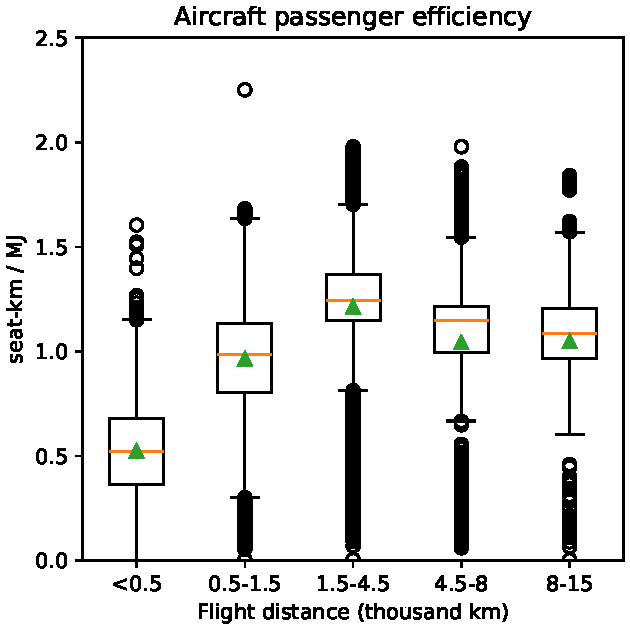
\includegraphics[width=\columnwidth]{figs_models/current_aircraft_energy.pdf}
    \caption{Distribution of current passenger efficiency according to flight distance. Data from \cite{salgas_aeroscope}.}
    \labfig{current-energy}
\end{marginfigure}

\begin{marginfigure}
    \centering
    
\includegraphics[width=\columnwidth]{figs_models/current_aircraft_lifetime.pdf}
    \caption{Distribution of aircraft age at retirement according to number of seats. Data from \cite{planespotters}.}
    \labfig{current-lifetime}
\end{marginfigure}

The main properties of the current aircraft fleet are initialized based on data from the AeroSCOPE database \sidecite{salgas_aeroscope}. The database contains information (passengers flown, seating capacity, fuel burn, emissions) for each origin-destination route for the year 2019 (\reffig{current-histograms}). This is then used in order to estimate the share of global traffic per market segment (supposed to stay constant in time), and also the energy consumption of a typical aircraft within a market.

It is further assumed that, within a given market segment, aircraft can only be replaced by a new aircraft architecture tailored for this market. As shown in \reffig{current-energy}, there are significant discrepancies in the aircraft passenger efficiency (the inverse of the energy consumption per seat-km) for flights within the same market segment, and which are higher over short distance flights, meaning that aircraft used for these are not optimized for these distances.

To account for this, the energy consumption initialized for the current fleet is dependent on the technology scenario: the Lower technology considers the lower quartile in terms of passenger efficiency, the Mid technology considers the median, and the Upper technology considers the upper quartile.

At last, the lifetime of the current aircraft fleet are initialized based on data from the \textit{planespotters} database \sidecite{planespotters}. Instead of aggregating market segments based on distances, aircraft are aggregated by number of seats for closer alignment with aircraft design classes, and it is assumed that, within a market aircraft are subject to the same fleet replacement dynamics. \reffig{current-lifetime} shows how the age of retired aircraft is distributed, within each segment the distribution is positively skewed (median is lower than mean), but there are significant discrepancies within and across markets. The fleet lifetimes are also dependent on technology scenario: the Lower technology considers the upper quartile in terms of lifetime, the Mid technology considers an intermediate value, and the Upper technology considers the median value. The lower quartile is not used, as the median value is already below the mean, and therefore already a more optimistic value than currently. For comparison, values used for fleet replacement lifetimes in analogous studies \sidecite{grewe_evaluating_2021, kar_dynamics_2009, delbecq-fleet} are, respectively, 15, 20, and 25 years.

\begin{table*}[t!]
    \caption{TLAR determined by market segment.}
    \centering
    \begin{tabular}{c|c c|cc}
    \toprule
    Market & Range (km)  & Seats & Consumption (MJ/seat-km) & Lifetime (years)\\
    \midrule
    General & 500 & 19 & 2.74-1.47 & 33.8-22.2\\
    Commuter & 1500 & 50 & 1.25-0.88 & 26.5-21.9\\
    Regional & 4500 & 80 & 0.87-0.73 & 20.5-15.3\\
    Short-medium & 8000 & 120 & 1.00-0.82 & 33.8-24.8\\
    Long range & 15000 & 250 & 1.03-0.83 & 29.5-23.6\\
    \bottomrule
    \end{tabular}
    \label{tab:tlar-category}
\end{table*}

Table \ref{tab:tlar-category} summarizes how market segments are split into aircraft range and number of seats, as well as the assumptions on vehicle consumption and lifetime initialized for the market (the last two being dependent on the technology scenario chosen).

\begin{figure*}[b!]
    \centering
    
\includegraphics[width=1.5\textwidth]{figs_models/aircraft_technology.pdf}
    \caption{Improvement in selected aircraft parameters as a function of expected Entry-Into-Service. Filled between the upper and lower limit for the technology scenarios, solid line shows lower technology scenario, and dotted line shows mid technology scenario.}
    \labfig{aircraft-tech}
\end{figure*}

\subsection{Prospective aircraft design}
\label{subsec:aircraft-design}

Modifying the energy carrier changes and the propulsion system architecture requires specific technology, e.g., cryogenic fuel tank, fuel cells, electric motors, all of which are expected to mature at different rates.

To demonstrate this, several sources are used to provide technology parameters and expected year of entry-into-service, which include research papers on green transportation technologies \sidecite{wallington_green_2024, adler_energy_2025} technology roadmaps from IATA \sidecite{iata_tech_2050} and ATI \sidecite{ati_aerodynamic, ati_cryogenic, ati_electrical, ati_fuelcell}, ICCT aircraft design studies \sidecite{icct_hydrogen, icct_electric, icct_fuelcell}  NASA electric propulsion studies and technology aspiration \sidecite{felder_nasa_2015, papathakis_nasa_2017, woodworth_nasas_nodate, bradley_subsonic_2015} and EASA type certificate data \sidecite{easa234}.

Table \ref{tab:aircraft-tech} presents the lower and upper values used for the technology parameters, according to entry-into-service (EIS) and Figure \reffig{aircraft-tech} displays how some key parameters are interpolated in time and how they compare with the sources used. The main goal of this is to be able to account for the trade-off regarding the timing of deployment of aircraft architectures: early deployment of maturing technology and lock-in with mediocre performance, or late deployment with mature and better performances. \reffig{aircraft-tech} compares the values used in the present work with the literature depending on expected year of Entry-Into-Service.

In order to avoid over-reliance on optimist technology, especially in a sector that has missed many of its recent environmental targets \sidecite{missed-targets}, some sources that are purposefully left out of the technology scenario range. This is of particular importance for fuel-cell systems because:

\begin{itemize}
    \item Fuel-cells have limited power output, so several cells have to be stacked to compose total power, decreasing power-to-weight ratio of the system;
    \item Narrow ranges of operating temperature plus high thermal losses, means these systems require thermal management for high-power applications, adding further weight (which is included in the fuel-cell specific power);
    \item Aircraft-tailored applications needs much higher power output relative to automotive fuel cells, overall studies may display diverging assumptions on whether the larger scale will result in improved \cite{icct_fuelcell} or degraded efficiency performance \sidecite{seitz_initial_2022}.
\end{itemize}

The Top-Level Aircraft Requirements (TLAR) are split into two sets: the number of seats and range are determined solely by the market segment (Table \ref{tab:tlar-category}), the cruise speed and altitude are determined by the propulsion architecture (Table \ref{tab:tlar-architecture}). Overall, gas turbines can yield efficient operation at higher and faster flight conditions relative to propellers, but their cruise altitude and speed were purposefully limited in the present work, based on recent findings that re-designing aircraft to fly lower and slower can significantly reduce non-CO2 impacts at less than 1 \% extra operating cost \sidecite[][Figures 6.5, 6.8, 6.13, and Table E.4]{proesmans_thesis_2024}.

\begin{table*}[t!]
    \caption{Quantitative evolution of aircraft technology parameters.}
    \centering
    \begin{tabular}{c|c|c c c|c}
    \toprule
    Technology Parameter & Unit  & 2020 & 2040    & 2060     & Sources   \\
    \midrule
    Battery Specific Energy     & Wh/kg & 200  & 350-800 & 600-1500 & \cite{iata_tech_2050, icct_electric, felder_nasa_2015, bradley_subsonic_2015, woodworth_nasas_nodate} \\
    E-motor Specific Power      & kW/kg & 2    & 10-25   & 15-28 & \cite{ati_electrical, papathakis_nasa_2017} \\
    Electronics Specific Power  & kW/kg & 2    & 15-25   & 20-32 & \cite{ati_electrical, woodworth_nasas_nodate} \\
    Fuel cell Specific Power    & kW/kg & 1    & 2-3     & 3-6 & \cite{iata_tech_2050, ati_fuelcell, papathakis_nasa_2017, wallington_green_2024} \\
    Fuel cell Efficiency        & \%    & 40  & 45-55   & 50-65 & \cite{ati_fuelcell, wallington_green_2024} \\
    LH2 tank Gravimetric Index  & \%    & 20   & 30-65   & 35-80 & \cite{iata_tech_2050, ati_cryogenic, icct_hydrogen, icct_fuelcell, wallington_green_2024} \\
    Structural weight reduction & \%    & 0    & 15-30   & 20-40 & \cite{iata_tech_2050, ati_aerodynamic} \\
    \bottomrule
    \end{tabular}
    \label{tab:aircraft-tech}
\end{table*}

The Generic Airplane Model (GAM) \sidecite{kambiri_energy_2024}, from ENAC, is then used as a preliminary airplane design tool. It uses regression of historical airplane data to estimate airframe and structural weight and adds the propulsion system mass depending on the technology components that each architecture uses.

\begin{table}[h!]
    \caption{TLAR determined by aircraft architecture.}
    \centering
    \begin{tabular}{c|c c}
    \toprule
    \multirow{2}{*}{Architecture} & Speed & Altitude\\
    & (Mach) &  (thousand ft)\\
    \midrule
    Jet-A and Gas Turbine & 0.75 & 27 \\
    LH2 and Gas Turbine & 0.75 & 27 \\
    % Turboprop & 0.5 & 20000 \\
    Battery and E-motor & 0.5 & 20 \\
    LH2 fuel-cell and E-motor & 0.5 & 20 \\

    \bottomrule
    \end{tabular}
    \label{tab:tlar-architecture}
\end{table}

\subsection{Fleet deployment}

The global aircraft fleet is segmented into distance bands, rather than regionally or by routes. The 2019 repartition of ASK and emissions obtained from the AeroSCOPE database \sidecite{salgas_aeroscope} are also used to compare current energy consumption to that of new aircraft designs.

% \begin{figure}
%     \centering
%     \includegraphics[width=0.95\columnwidth]{figs_models/histogram_ask.pdf}
%     \caption{Histogram of the repartition of Available Seat-Kilometers according to flight distance of 2019 flights. Dark lines represent the repartition of distance among categories. Source: \cite{salgas_aeroscope}.}
%     \labfig{histo-ask}
% \end{figure}

% \begin{figure}
%     \centering
%     \includegraphics[width=0.95\columnwidth]{figs_models/histogram_co2.pdf}
%     \caption{Histogram of the repartition of CO2 emissions (kg) according to flight distance of 2019 flights. Dark lines represent the repartition of distance among categories. Source: \cite{salgas_aeroscope}.}
%     \labfig{histo-co2}
% \end{figure}

\begin{equation}
\label{eq:segmented-avoidance}
\begin{split}
    ASK(t) & = \sum_{m\ in\ \text{markets}} ASK_m(t)\\
    & =\sum_{m\ in\ \text{markets}} S_{m}\ ASK_{trend}(t)\ (1 - SR_{m} (t) )
\end{split}
\end{equation}

Each market is assigned a constant share of trend supply, and subject to a demand-side policy that avoids part of the trend demand (Eq. \ref{eq:segmented-avoidance}). The Supply-Shift Ratio $SR$ is treated as a time-dependent control, whose input values are used as optimization variables in the low-demand formulation, and it represents the part of trend supply that is to be avoided ($0$: all trend supply is met, $1$: all flights are banned).

\begin{equation}
    \label{eq:elast_price}
    \frac{dp}{p}=\frac{1}{\epsilon_p}\frac{dD}{D} \implies \ln\left(\frac{p_{cap}}{p_{trend}}\right) = \frac{1}{\epsilon_p} \ln\left(\frac{D_{cap}}{D_{trend}}\right)
\end{equation}

In Equation \ref{eq:burden-time}, the annual burden associated to demand aversion is defined, formulated as the relative ticket price increase due to the chosen value for $SR$. Under the assumptions that: demand reduction ultimately increase consumer prices (either caused by a tax or as a consequence of scarce supply), price elasticity $\epsilon_P$ is constant in time and among markets. From the definition of price elasticity $\epsilon_p=\frac{dRPK/RPK}{dp/p}$, one can derive by integration (Eq. \ref{eq:elast_price}) that the relative ticket price change is equal to $(1-SR)^{1/\epsilon_p}$ to the relative demand change. While the assumptions are not applicable to reality due to market-specific elasticities \sidecite{iata-elasticities}, they may still serve as simplified way to compare the suitability of scenarios with demand-aversion strategies without recurring to cost estimations.

In Equation \ref{eq:burden-avoidance}, the objective function of the low-demand formulation is defined as the present valuation of future policy burdens. It is a time-integration of the annual burden of demand avoidance, multiplied by a discount factor. The social discount rate $d_f$ is the rate at which future burdens are undermined relative to present burdens, which was set at 3 \%. There is, however, a significant debate \sidecite{goulder_choice_2012, schoenmaker_which_2024} on whether this parameter should be defined by normative (how policies should be put in place) or positive (how policies likely will be put in place) approaches, the value chosen stands as a middle ground between the normative and the positive range.

\begin{equation}
\label{eq:burden-time}
    \theta_{avoidance}(t) = \frac{\Delta P}{P} = \frac{\sum_{m\ in\ \text{markets}} S_m \left(1-SR_m(t)\right)^{1/\epsilon_p}}{ASK(t)}
\end{equation}

\begin{equation}
\label{eq:burden-avoidance}
\begin{split}
    \Theta_{avoidance} = & \int_{t_0}^{t_1} (1+ d_f)^{t_0-t}\ \theta_{avoidance}(t)\ dt
\end{split}
\end{equation}

\begin{marginfigure}
    \centering
    
\includegraphics[clip, trim=0cm 0cm 0cm 16.7cm, width=\columnwidth]{figs_models/first-order-delay.pdf}
    \caption{Fleet deployment of new aircraft concepts is modeled as a delayed response to a ramped pulse signal, controlled by $EIS, S\text{max}, t_{ramp}, t_{lifetime}$}
    \labfig{fleet-controls}
\end{marginfigure}

The market share of each aircraft type is also modeled using time-dependent controls (Eq. \ref{eq:delay}), but subject to a parameterized ramped pulse shape. The input signal is treated as zero before the year of Entry-Into-Service EIS, and then grows from 0 to a max share $S\text{max}$ linearly for a duration of $t_{ramp}$. EIS and $S\text{max}$ are tailored for each aircraft design and used as optimization variables. $t_{ramp}$ is parameterized as $2\tau_{fleet}$ to maintain the ramped step shape, and $\tau_{fleet}$ is determined by current market lifetime.

\marginnote{
\begin{equation}
    C_{aircraft} (t) = ASK_{aircraft}(t) EC_{aircraft}
    \label{eq:aircraft-consumption}
\end{equation}
}
The total energy carrier consumed by aircraft operations is estimated from covered supply and design energy consumption (sub-section \ref{subsec:aircraft-design}) as shown in Equation \ref{eq:aircraft-consumption}. Then, the direct consumption of each energy carrier is aggregated as the sum among the carrier-consuming aircraft in Equation \ref{eq:aircraft-aggregation}.

\begin{equation}
    C\text{direct}_{\text{energy}} = \sum_{a\ in\ \text{energy architectures}} C_{a}
    \label{eq:aircraft-aggregation}
\end{equation}

% \begin{equation}
%     ASK_{aircraft} (t) = ASK_{market}(t) \frac{S\text{max}_{aircraft}}{1+\exp{\left(-k(t-\tau))\right)}}
%     \label{eq:aircraft-supply}
% \end{equation}

% \begin{equation}
%     k = \frac{\log{100}}{LT/2}
%     \label{eq:aircraft-k}
% \end{equation}
% \begin{equation}
%     \tau = EIS_{aircraft}-\frac{LT}{2}
%     \label{eq:aircraft-tau}
% \end{equation}

\subsection{Energy-Mix}

This work considers different energy carriers, and for some of them several production pathways are available, such as synthetic fuels. Moreover, some energy carriers can be consumed in the production of other carriers and some of them can compete for the same primary energy sources or materials. In that regards, it is necessary to consider a modular implementation to the energy production model.

Each energy conversion process is modeled in a modular manner as a production pathway. Pathways have a specific consumption of input flows per unitary production of output flows. The energy mix assembles all the production processes and the links them to calculate both intensive and extensive properties of the energy production system.

The computation of the impact generated (only CO2 emissions in this work, but any cumulative impact could be extended, such as land required, water consumption, ...) per unitary production, an intensive quantity, is made from primary-to-final. This is mainly due to the fact that the impacts made in the production of inputs must be known beforehand in order to be accounted for in the indirect impacts of outputs. On the other hand, the aggregated consumption and production of energies, an extensive quantity, is made from final-to-primary, because total consumption of final energies determine the required consumption of inputs, which determines how much production of each energy-input is required.

% Consider the energy system required to produce two final energy carriers: Jet-A and liquid hydrogen. Jet-A is produced from a mix of fossil kerosene, and synthetic kerosene (electrofuel). Gaseous hydrogen is produced from electrolysis and is used to produce both liquid hydrogen, through liquefaction, and electrofuel, through power-to-liquid pathways.
% The emission factor ($EF$) of electrofuel and liquid hydrogen are both dependent on the $EF$ of gaseous hydrogen, which depends on that of electricity. The computation of $EF$ starts with electricity (primary), then gaseous hydrogen (secondary), then liquid hydrogen (final) and electrofuel (secondary), then Jet-A (final). The total production of each energy, however, must follow the inverse path: from final-to-primary. Taking the same example: Power-to-liquid production depends on Jet-A consumed, and liquefaction production depends on liquid hydrogen consumed. Electrolysis production depends on the gaseous hydrogen consumed in liquefaction and power-to-liquid production. Finally, electricity production required is estimated from consumption in the production of gaseous hydrogen. The computation of aggregated production and consumption starts with Jet-A (final) and liquid hydrogen (final), then electrofuel (secondary), then gaseous hydrogen (secondary), then electricity (primary).

In some implementations of modular energy system models, the estimation of properties is made altogether (intensive and extensive) per energy type and pathway \sidecite{witness}. This creates a coupled model: intensive quantities depend on the mix of the upstream system and extensive quantities depend on the aggregated consumption of the downstream system. This yields that an initial guess must be made up- and downstream, which is then iteratively solved until convergence. By separating modules responsible for estimating intensive and extensive quantities, if the system has no retroaction, the coupling disappears and direct computation can be achieved.

% (Figure \reffig{energy-mix-altogether})
% (Figure \reffig{energy-mix-separate})

% \begin{figure*}
%     \centering
%     \includegraphics[width=0.55\textwidth]{figs_models/altogether.png}
%     \caption{Coupling graph of the energy-mix models when using one module per energy type. This graph has two way couplings and require iterative processes to be solved.}
%     \labfig{energy-mix-altogether}
% \end{figure*}

% \begin{figure*}
%     \centering
%     \includegraphics[width=\textwidth]{figs_models/separate.png}
%     \caption{Coupling graph of the energy-mix models when using two modules (impact and consumption) per energy type. This graph has no two way couplings and can be solved sequentially.}
%     \labfig{energy-mix-separate}
% \end{figure*}

\subsubsection{Intensive impacts}

\begin{table*}[b!]
    \caption{Energy consumption and direct emissions for each of the production pathways considered. For pathways under technology maturing, the two values represent the 2025 and 2050 values.}
    \footnotesize
    \centering
    \begin{tabular}{c c|c c c c|c|c}
    \toprule
    \multirow{2}{*}{Energy Carrier} & \multirow{2}{*}{Production Pathway}  & \multicolumn{4}{c|}{Energy consumption (MJ/MJ)} & Direct emissions  & \multirow{2}{*}{Source}   \\
    & & Oil & Biomass & Electricity & Gas H2 & (g CO2 / MJ) & \\
    \midrule
    Fossil Jet-A & Refinery & 1.16 & - & - & - & 88.7  &  \cite{jing_understanding_2022} \\
    \hline
    \multirow{3}{*}{Biofuel} & HEFA & - & 1.95 & - & - & 62.73 & \multirow{3}{*}{\cite{NEULING201854}} \\
    & ATJ & - & 3.33 & - & - & 51.55 & \\
    & FT & - & 5.0 & - & - & 35.3 & \\
    \hline
    \multirow{2}{*}{Gas H2} & Gas reforming & - & - & - & - & 101.5 & \cite{ji_h2} \\
    \cline{8-0}
     & Electrolysis & - & - & 1.41-1.33 & - & 0 & \multirow{3}{*}{\cite{wallington_green_2024}} \\
    \cline{1-7}
    Electrofuel & Power-to-liquid & - & - & 0.65-0.56 & 1.89-1.68; & 0  &   \\
    \cline{1-7}
    Liquid H2 & Liquefaction &  - & - & 0.22-0.16 & 1.0 & 0 &  \\
    \bottomrule
    \end{tabular}
    \label{tab:energy-prod}
\end{table*}

% \begin{table*}
%     \caption{Emission factor associated to energy inputs and brief description of the method to estimate them. For pathways under technology maturing, the two values represent the 2025 and 2050 values.}
%     \centering
%     \begin{tabular}{c|c|c c}
%     \toprule
%     \multirow{2}{*}{Energy input} & Emission factor & \multirow{2}{*}{Method} & \multirow{2}{*}{Source}\\
%      & (g CO2 / MJ) & & \\
%     \midrule
%     Oil & 63.32 & Kerosene combustion divided by oil consumption & \cite{stratton_impact_2011}\\
%     Biomass & 0 & Accounted only as biofuel direct emissions & \cite{NEULING201854}\\
%     Electricity & Scenario-dependent & Final consumption divided by electricity emissions & \cite{ar6_database}\\
%     \bottomrule
%     \end{tabular}
%     \label{tab:energy-input}
% \end{table*}

Impacts generated in the production of energy carriers are heavily dependent on the efficiency of processes and the impacts of consumed inputs, and these are mainly determined by the background energy system \sidecite[-80pt]{mendoza_beltran_when_2020}. Recent works have highligthed the importance of linking global scenarios to perform prospective life-cycle assessment of energy \sidecite[-50pt]{sacchi_premise_2022}, and have also been applied for the prospective assessment of climate neutral aviation \sidecite{sacchi_how_2023}, showing a great increase in emissions associated with the production of synthetic jet fuel when a 3.5°C temperature increase scenario is chosen instead of a 2°C one.

The impact factor $IF_{\text{pathway}}$ (Eq. \ref{eq:impact-pathway}), impact per unitary production, of each output flow associated to production pathways is modeled as the sum of direct impact generated at production plus the impacts associated to the input flows consumed in the process. $CF_{p, i}$ is the consumption of input $i$ per unitary production of pathway $p$. This is made because the inputs consumed in the process have impacts themselves, and by consuming them these indirect impacts must be accounted in the impacts of the output flow.

Table \ref{tab:energy-prod} summarizes the production pathways for each of the accounted energy carriers, their energy consumption and direct emissions per produced output. Technology maturing was accounted for some production pathways with an inverse consumption (analogous to process efficiency) that decreases linearly until stagnation in 2050.

% \begin{figure}
%     \centering
%     \includegraphics[width=\columnwidth]{figs_models/electricity_co2_intensity.pdf}
%     \caption{Emission factor associated to electricity consumption depending on the chosen background scenario. Source \cite{ar6_database}.}
%     \labfig{electricity-emission}
% \end{figure}

\begin{equation}
\label{eq:impact-pathway}
\begin{split}
    IF_{\text{pathway}}= & IF\text{direct}_{\text{pathway}}\\
    &+\sum_{i\ in\ \text{pathway inputs}}CF_{\text{pathway}, i}\ IF_i
\end{split}
\end{equation}

\marginnote{
\begin{equation}
    IF_{\text{energy}}=\sum_{p\ in\ \text{energy pathways}}S_p\ IF_p
    \label{eq:impact-energy}
\end{equation}
}

Because each energy type can be produced by several pathways, a mixing process is applied where the energy mean impacts $IF_{\text{energy}}$ (Eq. \ref{eq:impact-energy}) is weighted by the share of pathway production, which are treated as a time-dependent control, used as optimization variables.

\subsubsection{Extensive production and consumption}

The production of each energy type (Eq. \ref{eq:prod-energy}) is the direct energy consumption (directly embarked in aircraft) plus what was consumed to make other energy types. If $e_0$ is an energy input to $e_1$, $e_1$ is an energy output to $e_0$. The computation is initialized with final energies because the term $\sum_{o}(CF_{o, e}\ P_o)$ is zero, as no intermediate processes consume them.

\begin{equation}
    P_{\text{energy}}=C\text{direct}_{\text{energy}} + \sum_{o\ in\ \text{energy outputs}}CF_{o, \text{energy}}\ P_o
    \label{eq:prod-energy}
\end{equation}

\marginnote{
\begin{equation}
    P_{\text{pathway}}=S_{\text{pathway}}\ P_{\text{energy}}
    \label{eq:prod-pathway}
\end{equation}
}

The production of each pathway (Eq. \ref{eq:prod-pathway}) is then estimated from pathway share. Input consumption of pathways are estimated (Eq. \ref{eq:cons-pathway}) and then are aggregated by energy type (Eq. \ref{eq:cons-energy}). The process is then repeated for each energy type until primary energies.

\begin{equation}
    C_{\text{pathway}, \text{input}}=CF_{\text{pathway}, \text{input}}\ P_{\text{pathway}}
    \label{eq:cons-pathway}
\end{equation}

\marginnote{
\begin{equation}
    C_{\text{energy}, \text{input}}=\sum_{p\ in\ \text{pathways}} C_{p, \text{input}}
    \label{eq:cons-energy}
\end{equation}
}

\subsubsection{Consumption and impacts constraints}

For biomass and electricity, the total consumption is constrained applying the concept of an allocation principle, initially developed for Absolute Environmental Sustainability Assessments \sidecite{bjorn_framework_2019, hjalsted_sharing_2021}, but applied for energy production (Equation \ref{eq:conso_constraint}). Because there is little consensus on how to find such fair shares \sidecite{pais_current_2024}, two different values were explored: one reflecting a conservative energy availability (5.0 \%), and another reflecting a preferential availability to the aviation sector (8.6 \%). Both values use some sort of grandfathering, which tend to lock the economic system into its present state. Yet, values are still conservative when compared to other institutional roadmaps \sidecite{becken_implications_2023}.

\begin{equation}
    \label{eq:conso_constraint}
    C_{\text{resource}} \le s_{\text{resource}} P_{\text{resource}}
\end{equation}

The conservative value was obtained based on a reference mitigation scenario, the IMP-REN-2.0, in which 38.6 \% of the biomass production is allocated to the transport sector \sidecite{energy_ar6_wg3}, the fair share allocated to aviation is considered to be 13 \% of that, which is the 2019 sector's share of oil consumption relative to the entire transportation consumption \sidecite{IEA2019oil}. The preferential access value was obtained based on the sector's 2019 share of global oil consumption \cite{IEA2019oil}.

\begin{equation}
    \label{eq:co2_constraint}
    \int_{t_0}^{t_1} CO_2(t) dt \le s_{CO_2} B_{CO_2}
\end{equation}

In the low demand formulation, the cumulative emissions of the sector is a constraint rather than the objective to minimize (Eq. \ref{eq:co2_constraint}). In these cases, we assumed the target carbon budget $B_{CO_2}$ to be the remaining 2°C carbon budget with 66 \% confidence \sidecite{lamboll_assessing_2023}, and the fair share to be 3.0 \%, which is the sector's share of direct, indirect and induced GDP \sidecite{atag_benefits}.

\pagelayout{wide}

\section{Full scenario results}

\begin{figure*}[h!]
    \centering
    (a) Low technology:
    
\includegraphics[width=0.9\textwidth]{figs_results/single_policy/SSP2-26-Fossil-lowTech/fleet_SSP2-26-Fossil-lowTech.pdf}

    (b) Mid technology:
    
\includegraphics[width=0.9\textwidth]{figs_results/single_policy/SSP2-26-Fossil-midTech/fleet_SSP2-26-Fossil-midTech.pdf}

    (c) Upper technology:
    
\includegraphics[width=0.9\textwidth]{figs_results/single_policy/SSP2-26-Fossil-upTech/fleet_SSP2-26-Fossil-upTech.pdf}
    \caption{Fleet deployment for Baseline SSP2 scenarios.}
    \labfig{ssp2-fossil}
\end{figure*}


\begin{figure*}[h!]
    \centering
    (a) Low technology:
    
\includegraphics[width=0.8\textwidth]{figs_results/single_policy/SSP2-26-DropIn-lowTech/energy_SSP2-26-DropIn-lowTech.pdf}

    (b) Mid technology:
    
\includegraphics[clip, trim=0cm 8.5cm 0cm 0cm, width=0.8\textwidth]{figs_results/single_policy/SSP2-26-DropIn-midTech/energy_SSP2-26-DropIn-midTech.pdf}

    (c) Upper technology:
    
\includegraphics[width=0.8\textwidth]{figs_results/single_policy/SSP2-26-DropIn-upTech/energy_SSP2-26-DropIn-upTech.pdf}
    \caption{Energy-mix for the Drop-in trend scenarios.}
    \labfig{dropin-trend}
\end{figure*}

\begin{figure*}[h!]
    \centering
    (a) Low technology:
    
\includegraphics[clip, trim=0cm 8.5cm 0cm 0cm, width=0.8\textwidth]{figs_results/single_policy/SSP2-26-DropIn-Availability-lowTech/energy_SSP2-26-DropIn-Availability-lowTech.pdf}

    (b) Mid technology:
    
\includegraphics[width=0.8\textwidth]{figs_results/single_policy/SSP2-26-DropIn-Availability-midTech/energy_SSP2-26-DropIn-Availability-midTech.pdf}

    (c) Upper technology:
    
\includegraphics[clip, trim=0cm 8.5cm 0cm 0cm, width=0.8\textwidth]{figs_results/single_policy/SSP2-26-DropIn-Availability-upTech/energy_SSP2-26-DropIn-Availability-upTech.pdf}
    \caption{Energy-mix for the Drop-in availability scenarios.}
    \labfig{dropin-availability}
\end{figure*}

\begin{figure*}[h!]
    \centering
    (a) Fleet composition:
    
\includegraphics[width=\textwidth]{figs_results/single_policy/SSP2-26-DropIn-LowDemand-midTech/fleet_SSP2-26-DropIn-LowDemand-midTech.pdf}

    (b) Energy-mix:\\
    
\includegraphics[width=0.8\textwidth]{figs_results/single_policy/SSP2-26-DropIn-LowDemand-midTech/energy_SSP2-26-DropIn-LowDemand-midTech.pdf}
    \caption{Fleet composition and Energy-mix for the Drop-in low-demand scenario with Mid technology.}
    \labfig{dropin-lowdemand}
\end{figure*}


\begin{figure*}[h!]
    \centering
    (a) Low technology:
    
\includegraphics[clip, trim=0cm 10.7cm 0cm 0cm, width=\textwidth]{figs_results/single_policy/SSP2-26-lowTech/fleet_SSP2-26-lowTech.pdf}

    (b) Mid technology:
    
\includegraphics[clip, trim=0cm 10.7cm 0cm 0cm, width=\textwidth]{figs_results/single_policy/SSP2-26-midTech/fleet_SSP2-26-midTech.pdf}

    (c) Upper technology:
    
\includegraphics[clip, trim=0cm 6.5cm 0cm 0cm, width=\textwidth]{figs_results/single_policy/SSP2-26-upTech/fleet_SSP2-26-upTech.pdf}
    \caption{Fleet composition for the Breakthrough trend scenarios.}
    \labfig{break-trend-fleet}
\end{figure*}

\begin{figure*}[h!]
    \centering
    (a) Low technology:
    
\includegraphics[clip, trim=0cm 8.5cm 0cm 0cm, width=0.8\textwidth]{figs_results/single_policy/SSP2-26-lowTech/energy_SSP2-26-lowTech.pdf}

    (b) Mid technology:
    
\includegraphics[clip, trim=0cm 8.5cm 0cm 0cm, width=0.8\textwidth]{figs_results/single_policy/SSP2-26-midTech/energy_SSP2-26-midTech.pdf}

    (c) Upper technology:
    
\includegraphics[clip, trim=0cm 8.5cm 0cm 0cm, width=0.8\textwidth]{figs_results/single_policy/SSP2-26-upTech/energy_SSP2-26-upTech.pdf}
    \caption{Energy-mix for the Breakthrough trend scenarios.}
    \labfig{break-trend-energy}
\end{figure*}

\begin{figure*}[h!]
    \centering
    (a) Low technology:
    
\includegraphics[clip, trim=0cm 10.7cm 0cm 0cm, width=\textwidth]{figs_results/single_policy/SSP2-26-Availability-lowTech/fleet_SSP2-26-Availability-lowTech.pdf}

    (b) Mid technology:
    
\includegraphics[clip, trim=0cm 10.7cm 0cm 0cm, width=\textwidth]{figs_results/single_policy/SSP2-26-Availability-midTech/fleet_SSP2-26-Availability-midTech.pdf}

    (c) Upper technology:
    
\includegraphics[clip, trim=0cm 6.5cm 0cm 0cm, width=\textwidth]{figs_results/single_policy/SSP2-26-Availability-upTech/fleet_SSP2-26-Availability-upTech.pdf}
    \caption{Fleet composition for the Breakthrough availability scenarios.}
    \labfig{break-availability-fleet}
\end{figure*}

\begin{figure*}[h!]
    \centering
    (a) Low technology:
    
\includegraphics[clip, trim=0cm 8.5cm 0cm 0cm, width=0.8\textwidth]{figs_results/single_policy/SSP2-26-Availability-lowTech/energy_SSP2-26-Availability-lowTech.pdf}

    (b) Mid technology:
    
\includegraphics[clip, trim=0cm 8.5cm 0cm 0cm, width=0.8\textwidth]{figs_results/single_policy/SSP2-26-Availability-midTech/energy_SSP2-26-Availability-midTech.pdf}

    (c) Upper technology:
    
\includegraphics[clip, trim=0cm 8.5cm 0cm 0cm, width=0.8\textwidth]{figs_results/single_policy/SSP2-26-Availability-upTech/energy_SSP2-26-Availability-upTech.pdf}
    \caption{Energy-mix for the Breakthrough availability scenarios.}
    \labfig{break-availability-energy}
\end{figure*}

\begin{figure*}[h!]
    \centering
    (a) Low technology:
    
\includegraphics[clip, trim=0cm 10.7cm 0cm 0cm, width=\textwidth]{figs_results/single_policy/SSP2-26-LowDemand-lowTech/fleet_SSP2-26-LowDemand-lowTech.pdf}

    (b) Mid technology:
    
\includegraphics[clip, trim=0cm 10.7cm 0cm 0cm, width=\textwidth]{figs_results/single_policy/SSP2-26-LowDemand-midTech/fleet_SSP2-26-LowDemand-midTech.pdf}

    (c) Upper technology:
    
\includegraphics[clip, trim=0cm 6.5cm 0cm 0cm, width=\textwidth]{figs_results/single_policy/SSP2-26-LowDemand-upTech/fleet_SSP2-26-LowDemand-upTech.pdf}
    \caption{Fleet composition for the Breakthrough lowdemand scenarios.}
    \labfig{break-lowdemand-fleet}
\end{figure*}

\begin{figure*}[h!]
    \centering
    (a) Low technology:
    
\includegraphics[clip, trim=0cm 8.5cm 0cm 0cm, width=0.8\textwidth]{figs_results/single_policy/SSP2-26-LowDemand-lowTech/energy_SSP2-26-LowDemand-lowTech.pdf}

    (b) Mid technology:
    
\includegraphics[clip, trim=0cm 8.5cm 0cm 0cm, width=0.8\textwidth]{figs_results/single_policy/SSP2-26-LowDemand-midTech/energy_SSP2-26-LowDemand-midTech.pdf}

    (c) Upper technology:
    
\includegraphics[clip, trim=0cm 8.5cm 0cm 0cm, width=0.8\textwidth]{figs_results/single_policy/SSP2-26-LowDemand-upTech/energy_SSP2-26-LowDemand-upTech.pdf}
    \caption{Energy-mix for the Breakthrough lowdemand scenarios.}
    \labfig{break-lowdemand-energy}
\end{figure*}


\begin{figure*}[h!]
    \centering

    (a) SSP2-1.9:

    
\includegraphics[width=\textwidth]{figs_results/robust_policy/robust-SSP2-midTech/SSP2-19/fleet_SSP2-19.pdf}

    (b) SSP2-2.6:

    
\includegraphics[clip, trim=0cm 0cm 0cm 10.9cm, width=\textwidth]{figs_results/robust_policy/robust-SSP2-midTech/SSP2-26/fleet_SSP2-26.pdf}

    (c) SSP2-3.4:

    
\includegraphics[clip, trim=0cm 0cm 0cm 10.9cm, width=\textwidth]{figs_results/robust_policy/robust-SSP2-midTech/SSP2-34/fleet_SSP2-34.pdf}
    \caption{Fleet composition for the Scenario-robust trend scenarios.}
    \labfig{robust-trend-fleet}
\end{figure*}

\begin{figure*}[h!]
    \centering

    (a) SSP2-1.9:

    
\includegraphics[width=0.8\textwidth]{figs_results/robust_policy/robust-SSP2-midTech/SSP2-19/energy_SSP2-19.pdf}

    (b) SSP2-2.6:

    
\includegraphics[clip, trim=0cm 8.5cm 0cm 0cm, width=0.8\textwidth]{figs_results/robust_policy/robust-SSP2-midTech/SSP2-26/energy_SSP2-26.pdf}

    (c) SSP2-3.4:

    
\includegraphics[width=0.8\textwidth]{figs_results/robust_policy/robust-SSP2-midTech/SSP2-34/energy_SSP2-34.pdf}
    \caption{Energy-mix for the Scenario-robust trend scenarios.}
    \labfig{robust-trend-energy}
\end{figure*}

\begin{figure*}[h!]
    \centering
    (a) SSP2-1.9:
    
\includegraphics[width=\textwidth]{figs_results/robust_policy/robust-SSP2-lowdemand-LowDemand-midTech/SSP2-19/fleet_SSP2-19.pdf}

    (b) SSP2-2.6:
    
\includegraphics[width=\textwidth]{figs_results/robust_policy/robust-SSP2-lowdemand-LowDemand-midTech/SSP2-26/fleet_SSP2-26.pdf}

    (c) SSP2-3.4:
    
\includegraphics[width=\textwidth]{figs_results/robust_policy/robust-SSP2-lowdemand-LowDemand-midTech/SSP2-34/fleet_SSP2-34.pdf}
    \caption{Fleet composition for the Scenario-robust low-demand scenarios.}
    \labfig{robust-lowdemand-fleet}
\end{figure*}

\begin{figure*}[h!]
    \centering

    (a) SSP2-1.9:

    
\includegraphics[width=0.8\textwidth]{figs_results/robust_policy/robust-SSP2-lowdemand-LowDemand-midTech/SSP2-19/energy_SSP2-19.pdf}

    (b) SSP2-2.6:

    
\includegraphics[clip, trim=0cm 8.5cm 0cm 0cm, width=0.8\textwidth]{figs_results/robust_policy/robust-SSP2-lowdemand-LowDemand-midTech/SSP2-26/energy_SSP2-26.pdf}

    (c) SSP2-3.4:

    
\includegraphics[width=0.8\textwidth]{figs_results/robust_policy/robust-SSP2-lowdemand-LowDemand-midTech/SSP2-34/energy_SSP2-34.pdf}
    \caption{Energy-mix for the Scenario-robust trend scenarios.}
    \labfig{robust-lowdemand-energy}
\end{figure*}











% \blindtext

% \appendix % From here onwards, chapters are numbered with letters, as is the appendix convention

% \section{Appendix}

% \blindtext

%----------------------------------------------------------------------------------------
%	BIBLIOGRAPHY
%----------------------------------------------------------------------------------------

% The bibliography needs to be compiled with biber using your LaTeX editor, or on the command line with 'biber main' from the template directory

\printbibliography[title=Bibliography] % Set the title of the bibliography and print the references

\end{document}
